\section{Introduction}

\subsection{QCD phase structure}
%%%%%%%%%%%%%%%%%%%%%%%%%%%%%%%%%%%%%%%%%%%%%%%%%%%%%%%%%%%%%%%%%%%%%%%%%%%%%
\begin{frame}[fragile] % fragile is needed whenever verbatim env. is called.
    \begin{columns}
        \begin{column}{0.45\textwidth}
        Experiments:
            \begin{itemize}
            \item LHC Experiments at low density\\
            \item RHIC Beam Energy Scan at finite density\\
            \item ...
            \end{itemize}
        Goals:
            \begin{itemize}
            \item Location of Critical End Point (CEP)\\
            \item New phases at high density region \\
            \item EoS \\
            \item ...
            \end{itemize}
        \end{column}
        \begin{column}{0.5\textwidth}
            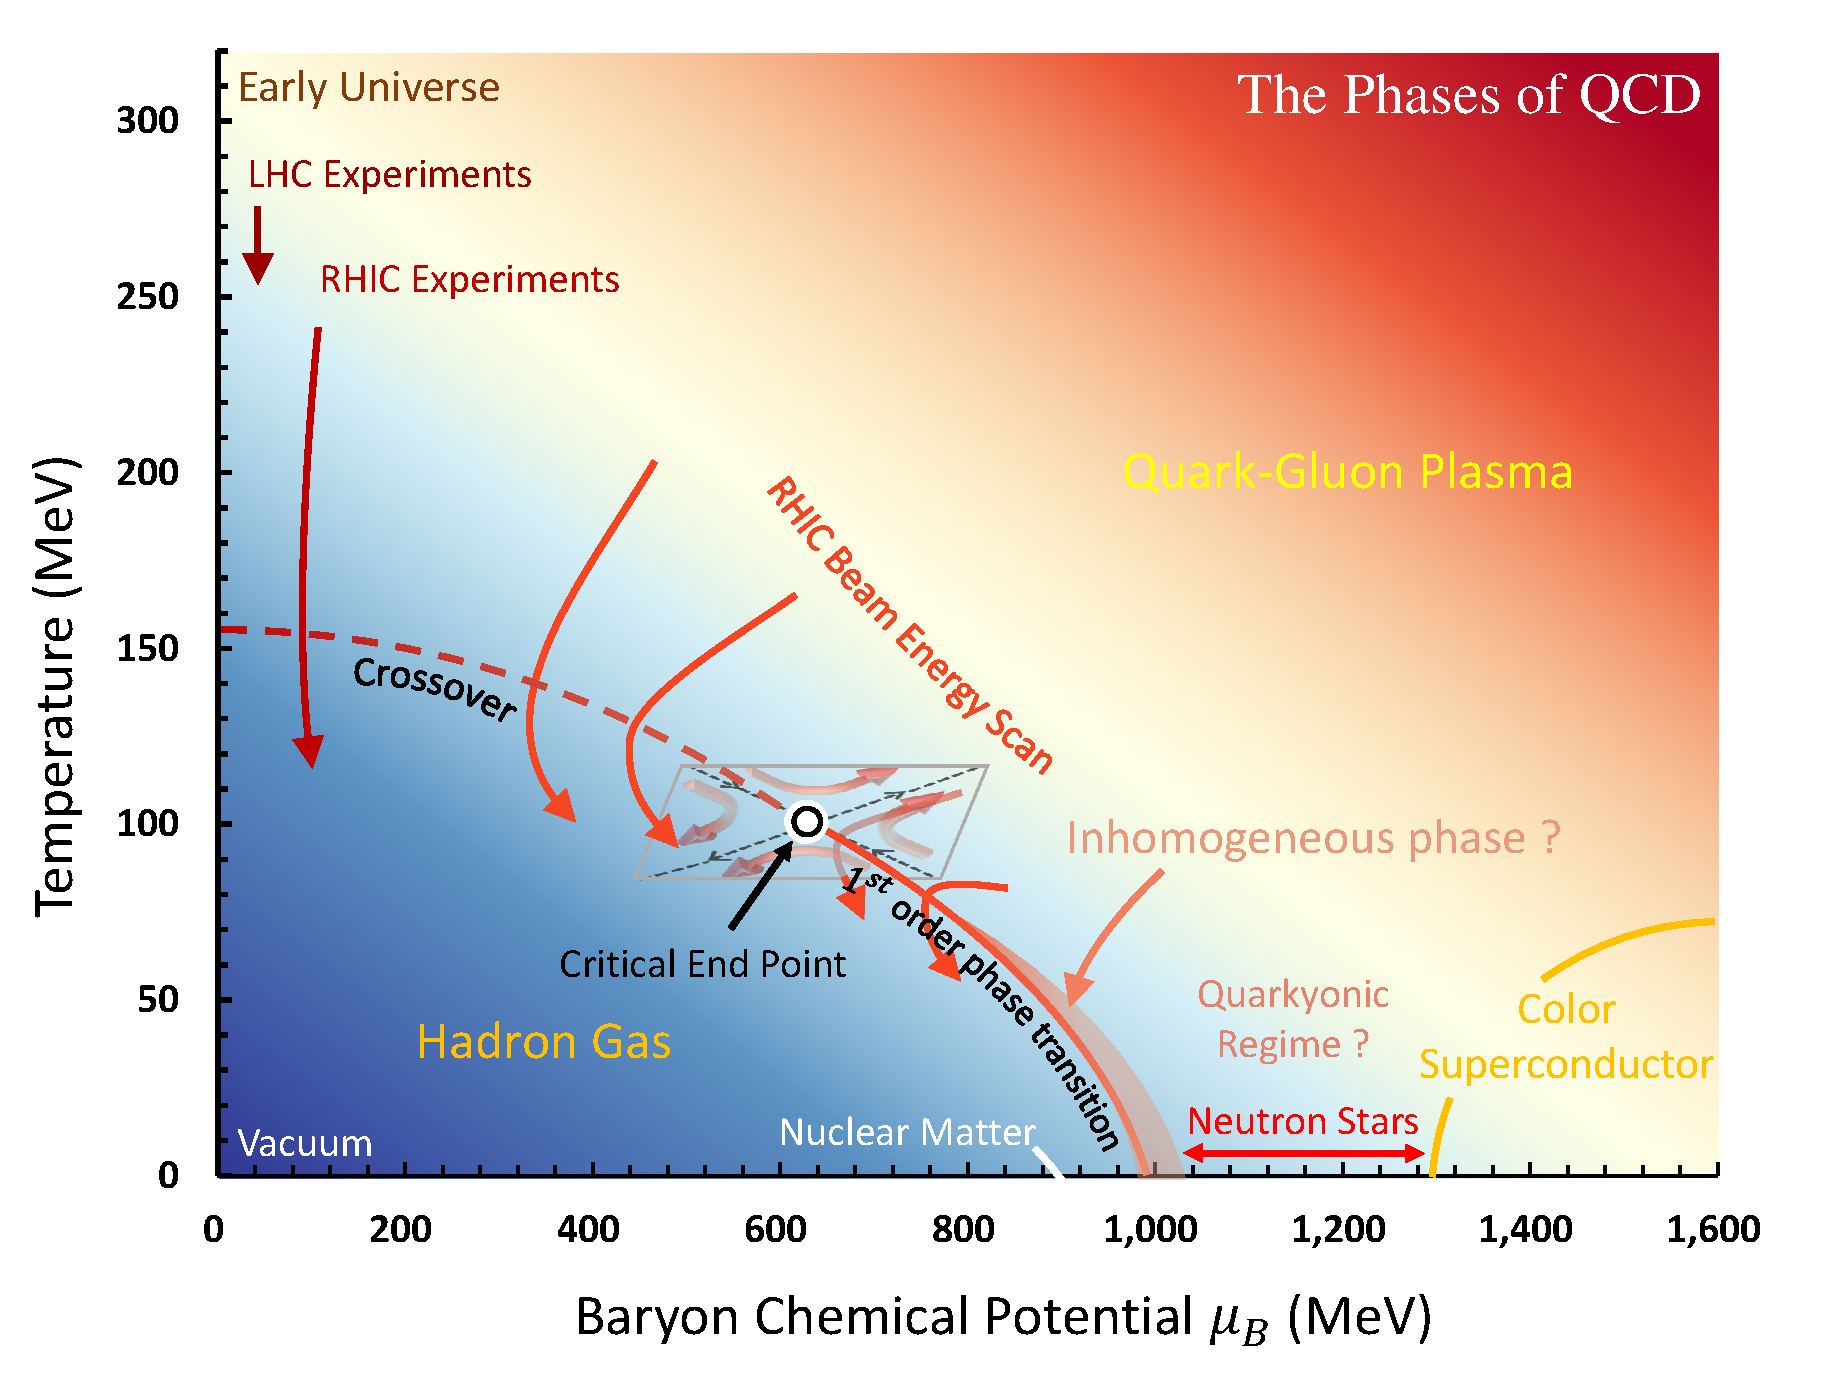
\includegraphics[width=1.15\linewidth]{Images/Figures/chap1_phase20240311.pdf}
            \vspace{-1.cm}
            \hspace{0.7cm}
            \hspace{1cm}{\scriptsize Nucl.Tech. 46 (2023) 04, 040002-040002}
            \vspace{1cm}
        \end{column}
    \end{columns}
\end{frame}
%%%%%%%%%%%%%%%%%%%%%%%%%%%%%%%%%%%%%%%%%%%%%%%%%%%%%%%%%%%%%%%%%%%%%%%%%%%%%
\begin{frame}[fragile]{Theoretical predictions}
    \begin{columns}
        \begin{column}{0.43\textwidth}
            \vspace{-7cm}
            \begin{itemize}
            \item Lattice QCD (at vanishing chemical potential)\\~\
            \item Dyson-Schwinger Equations (DSE)\\~\
            \item Functional renormalization group (fRG)\\~\
            \item ...
            \end{itemize}
        \end{column}
        \begin{column}{0.5\textwidth}
            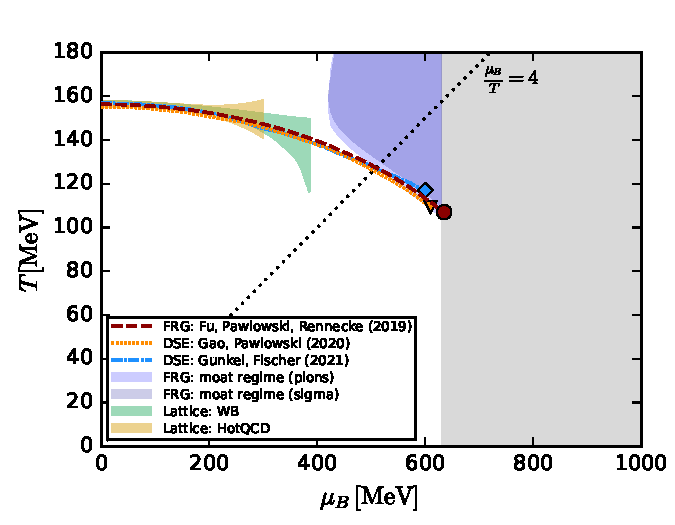
\includegraphics[width=1.15\linewidth]{Images/Figures/phasestructure_v4.pdf}
            \vspace{-0.8cm}
            \hspace{0.7cm}
            \hspace{2cm}{\scriptsize QCD phase diagram (fQCD 2025)}
            \vspace{8cm}
        \end{column}
    \end{columns}
\end{frame}
%%%%%%%%%%%%%%%%%%%%%%%%%%%%%%%%%%%%%%%%%%%%%%%%%%%%%%%%%%%%%%%%%%%%%%%%%%%%%
\begin{frame}[fragile]{Well known Advantages $\&$ Disadvantages}
    \vspace{-0.2cm}
    \begin{columns}
        \begin{column}{0.5\textwidth}
         \vspace{-1.29cm}
         \begin{block}{Lattice:}
            \begin{itemize}
            \item Reliable at 0 chemical potential\\~\
            \item Expansion methods are needed to reach finite density\\~\
            \end{itemize}
         \end{block}
         \vspace{0.8cm}
        \begin{itemize}
        \item Making reasonable use of reliable vanishing chemical potential results\\~\
        \item Attempt to reach higher chemical potentials
        \end{itemize}
        \end{column}
        \begin{column}{0.5\textwidth}
        \begin{block}{Functional methods:}
            \begin{itemize}
            \item Can compute at finite density\\~\
            \item Have to use truncations to prevent an infinite number of loop diagrams \\~\
            \end{itemize}
        \end{block}
        \hspace{0.5cm}
        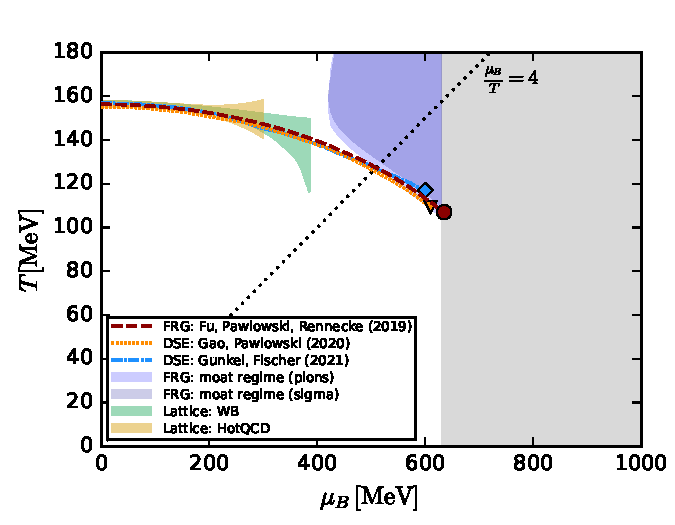
\includegraphics[width=0.82\linewidth]{Images/Figures/phasestructure_v4.pdf}
        \end{column}
    \end{columns}
\end{frame}
%%%%%%%%%%%%%%%%%%%%%%%%%%%%%%%%%%%%%%%%%%%%%%%%%%%%%%%%%%%%%%%%%%%%%%%%%%%%%
\subsection{Extrapolation to finite density}

\begin{frame}[fragile]
    \vspace{-0.2cm}
    \begin{block}{Taylor Expansion of the pressure:}
        \begin{align}
            \frac{p(T,\hat{\mu}_B)-p(T,0)}{T^4}=\sum^{\infty}_{n=1}\frac{1}{(2n)!}\chi^B_{2n}(T,0)\,\hat{\mu}_B^{2n}
        \end{align}
    \end{block}
    HotQCD: \hspace{7cm}WB:
    \vspace{0.5cm}
    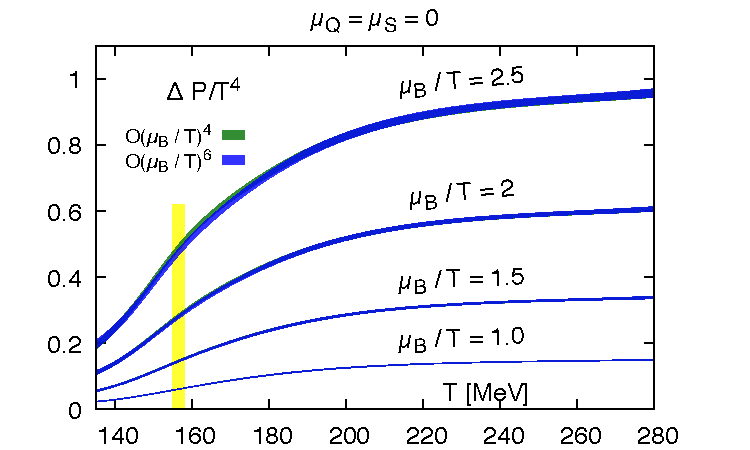
\includegraphics[width=0.5\linewidth,trim={0 0 0 0.6cm}, clip]{Images/Figures/Temp_BQS000_muB_Order_test.pdf}\hspace{1cm}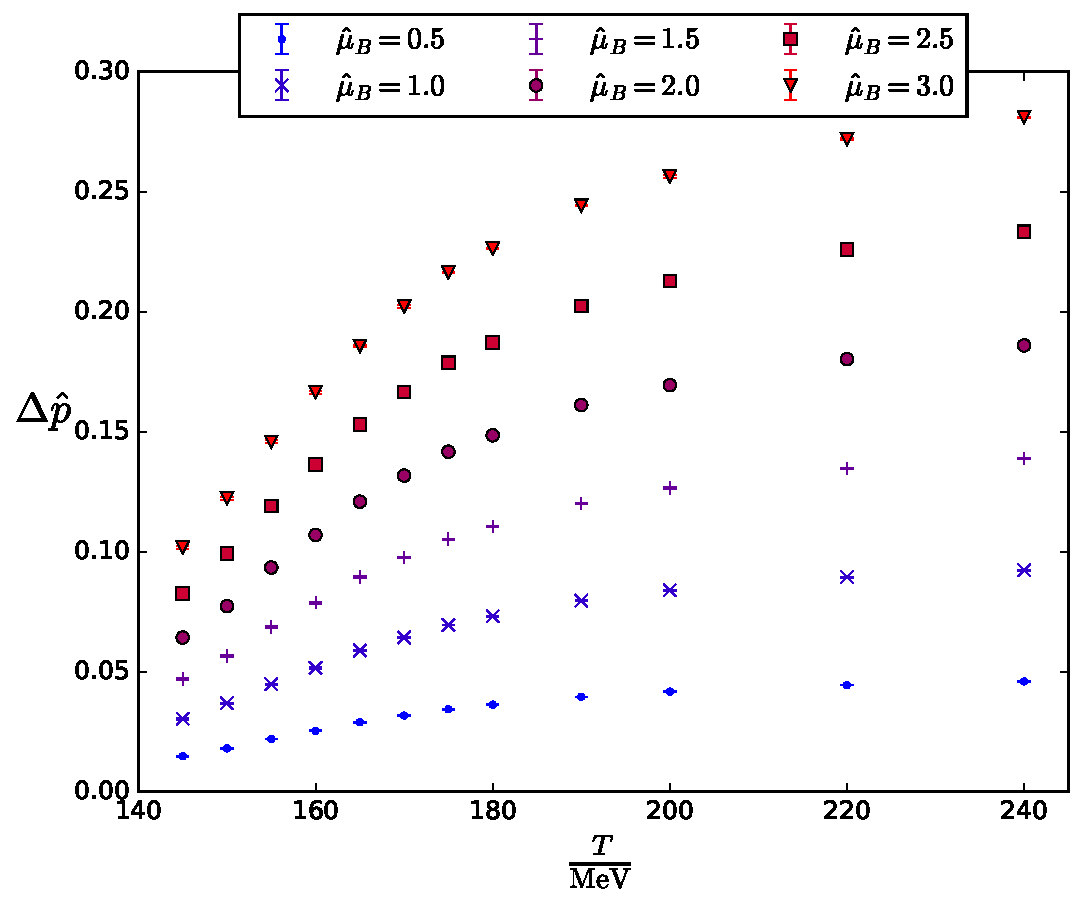
\includegraphics[width=0.4\linewidth,trim={0 1.3cm 0 0}, clip]{Images/Figures/plot6.pdf}
\end{frame}
%%%%%%%%%%%%%%%%%%%%%%%%%%%%%%%%%%%%%%%%%%%%%%%%%%%%%%%%%%%%%%%%%%%%%%%%%%%%%
\begin{frame}[fragile]{Extrapolation to finite density}
    \vspace{-0.2cm}
    \begin{block}{Pad\'{e} approximation:}
        \begin{align}
            P[m,n]=\frac{p(T,\hat{\mu}_B)-p(T,0)}{T^4}=\frac{\sum^{n/2}_{i=1}a_i\,\,\hat{\mu}_B^{2i}}{1+\sum^{m/2}_{j=1}b_i\,\,\hat{\mu}_B^{2j}}
        \end{align}
    \end{block}
    Here the coefficients $a_i$ and $b_i$ are determined by 
    \begin{align}
       \frac{\partial^iP[m,n]}{\partial\hat{\mu}_B^i}=\chi^B_i
    \end{align}
    \begin{itemize}
    \item When $m=0$ the Pad\'{e} approximation will go back to Taylor expansion
    \item The poles of Pad\'{e} approximation can be used to estimate the convergence radius of Taylor expansion
    \end{itemize}
\end{frame}
%%%%%%%%%%%%%%%%%%%%%%%%%%%%%%%%%%%%%%%%%%%%%%%%%%%%%%%%%%%%%%%%%%%%%%%%%%%%%
\begin{frame}[fragile]{Extrapolation to finite density}
    \vspace{-0.2cm}
    \begin{block}{Ratio estimator: (the pole of P[2,n])}
        \begin{align}
            r^{\mathrm{ratio}}_{c,2n}=\bigg| \frac{(2n+1)(2n+2)\chi^B_{2n}}{\chi^B_{2n+2}} \bigg|^{\frac{1}{2}}
        \end{align}
    \end{block}
    \begin{block}{Mercer-Roberts estimator: (the pole of P[4,n])}
    \begin{align}
            r^{\mathrm{MR}}_{c,2n}=&\bigg|\bigg[ \frac{\chi^B_{2n+2}\chi^B_{2n-2}}{(2n+2)!(2n-2)!}-\bigg(\frac{\chi^B_{2n}}{(2n)!}\bigg)^2 \bigg]\bigg|^{\frac{1}{4}}\,\,\bigg|\bigg[ \frac{\chi^B_{2n}\chi^B_{2n+4}}{(2n)!(2n+4)!}-\bigg(\frac{\chi^B_{2n+2}}{(2n+2)!}\bigg)^2 \bigg]\bigg|^{-\frac{1}{4}}
    \end{align}
    \end{block}
    \vspace{0.5cm}
    \begin{itemize}
    \item The estimators are given by the poles of the Pad\'{e} approximation 
    \item They can give a approximation convergence radius of Taylor expansion
    \end{itemize}
\end{frame}
%%%%%%%%%%%%%%%%%%%%%%%%%%%%%%%%%%%%%%%%%%%%%%%%%%%%%%%%%%%%%%%%%%%%%%%%%%%%%
\begin{frame}[fragile]{Extrapolation to finite density}
    \vspace{-0.2cm}
    \begin{block}{T' expansion:}
    \vspace{-0.2cm}
        \begin{align}
            \frac{\chi^B_1(T,\hat{\mu}_B)}{\hat{\mu}_B}&=\chi^B_2(T',0)\\
            T'(T,\hat{\mu}_B)=T\Big(1+\kappa_2(T)&\,\hat{\mu}_B^2+\kappa_4(T)\,\hat{\mu}_B^4+\mathcal{O}(\hat{\mu}_B^6)\Big)
        \end{align}
    \end{block}
    \vspace{0cm}
    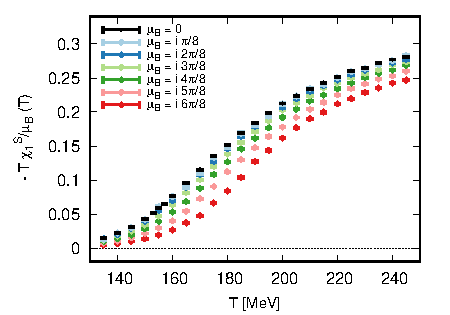
\includegraphics[width=0.47\linewidth,trim={0 0 0 0.28cm}, clip]{Images/Figures/shift_48x12_BS.pdf}\hspace{0.5cm}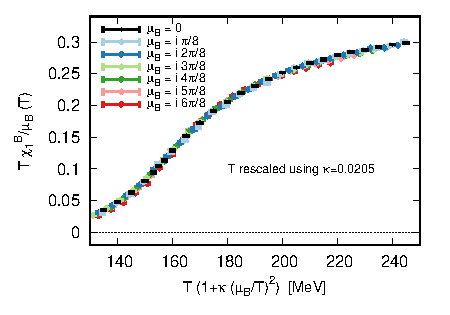
\includegraphics[width=0.48\linewidth,trim={0 0 0 0}, clip]{Images/Figures/shift_48x12_B2_collapse.pdf}\\
    \vspace{-0.3cm}{\centering \scriptsize Phys. Rev. Lett. 126, 232001 (2021) \par}
\end{frame}
%%%%%%%%%%%%%%%%%%%%%%%%%%%%%%%%%%%%%%%%%%%%%%%%%%%%%%%%%%%%%%%%%%%%%%%%%%%%%